\documentclass{article}
\usepackage{titlesec}
\usepackage{titling}
\usepackage[margin=1in]{geometry}
\usepackage{graphicx}
\author{iljo De Poorter}
\title{Software analyse les4}
\begin{document}
\maketitle
\section{Domeinmodelen software analyse}
Use case diagram, het bijhouden van alles over de use cases.

Waarom?
\begin{itemize}
\item Om goed te weten wat er aan de hand is met je project.
\item Om te weten wat je moet doen.
\item Visuele representatie van concepten uit de werkelijkheid, die we modeleren en waarvan we de onderlinge relatie tonen.
\end{itemize}
Er bestaan verschillende domeinklassen. Deze gebruiken we tot aan de kern van het probleem te geraken. 

Met hulp van het domeinmodel kan je nog steeds afstemmen met de klant of wij alles goed begrijpen.


Conceptuele klassen; domeinklassen, concepten uit de werkelijkheid die we modelleren.
Doel?
\begin{itemize}
\item Klassen om objecten uit de werkelijkheid te modeleren.
\item Mag enkel relevatne klassen bijhouden. == Geen DATATYPE. == GEEN BEREKENDEGEGEVENS.
\item naamgeving is opnieuw van belang(oosd) pascalCase.
\end{itemize}

\subsection{Voorbeeld}
Vliegtuig.
\begin{itemize}
\item VliegtuigID
\item VliegtuigType
\item aantalZitplaatsen
\item aantal(Vrije)Zitplaatsen
\end{itemize}


Kassier(persoon)
\begin{itemize}
\item KassierID
\item Naam
\item inDienstSinds
\item geboorteDatum
\end{itemize}

Winkel(filiaal)
\begin{itemize}
\item Naam
\item Adres
\end{itemize}

\subsection{Associaties}
Associetienaam, naam van de relatie tussen de klassen.
\begin{itemize}
\item Een verband tussen twee klassen/instances.
\item Enkel relevante data bijhouden.
\end{itemize}

Associetienaam
\begin{itemize}
\item Verduidelijking van de Associatie zelf.
\item Naamgeving is van belang, WERKWOORD, begin met hoofdletter.
\item Lezen van Links naar rechts, Boven naar onder.
\end{itemize}

Multipliciteit
\begin{itemize}
\item Aangeven hoeveel instanties van conceptuele klassen verbonden zijn met een andere conceptuele klasse.	
\item Hoeveel zijn er aanwezig PER ROL.
\item 1, 0..1, 0..*, 1..*, *..*, 1..n, n..m
\end{itemize}

\section{Oefeningen}
Verduidelijking bij rollen.
\begin{itemize}
\item Allen als associetienaam niet duidelijk is.
\item naamgaving is nogsteeds van belang.
\end{itemize}

\subsection{Oefening 1}
\begin{figure}[h]
  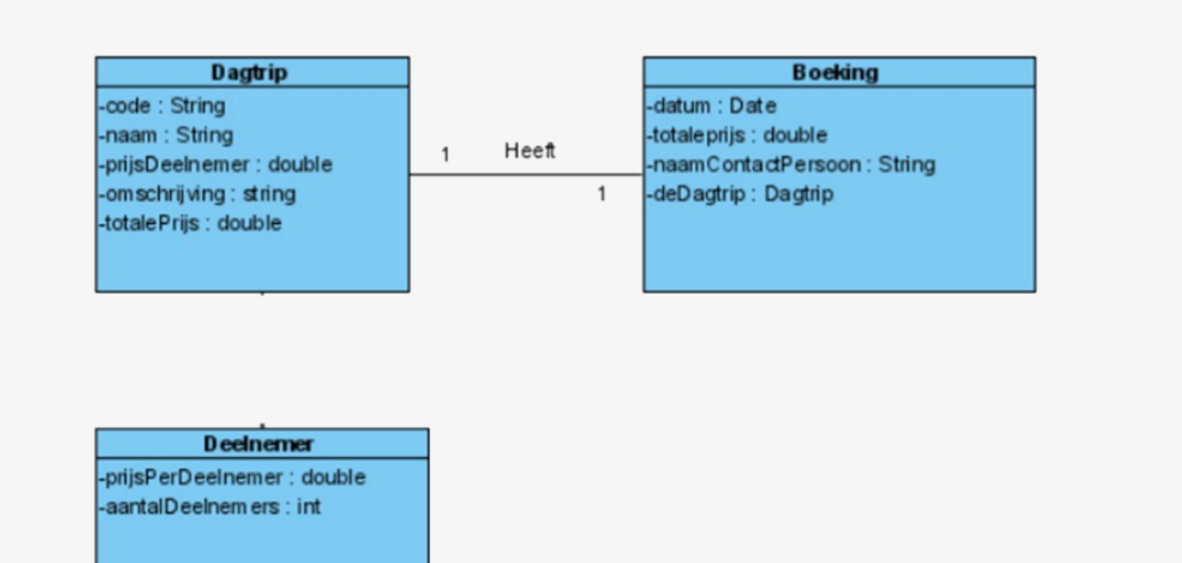
\includegraphics[width=0.6\linewidth]{oef1.png}
\end{figure}
Problemen
\begin{itemize}
\item Geen DATATYPEs in een domeinmodel. 
\item totaalPrijs is een berekend gegeven.
\item Totalprijs(boeking) is een berekend gegeven.
\item Attributen vn deelnemer zijn hier niet relevant. == Deelnemer mag weg.
\end{itemize}
Dagtrip -1---heeft---ok-Bezoek

Code			Datum

Naam			NaamCP

PrijsPP			AantalDeelnemers

Omschr
\subsubsection{Oefening 2}
\begin{figure}[h]
  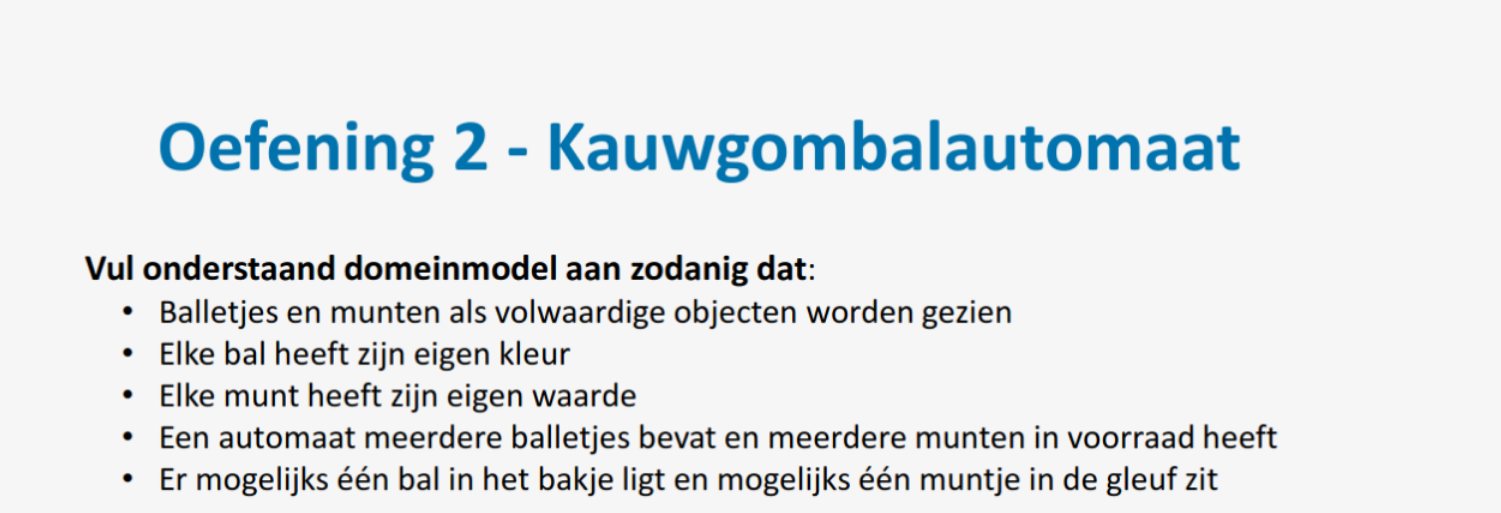
\includegraphics[width=0.6\linewidth]{oef2.png}
\end{figure}

KauwgombalAutomaat
\begin{itemize}
	\item Locatie???
\end{itemize}

KauwgombalAutomaat(0..1)---heeft---(0..*)munt

Munt
\begin{itemize}
	\item waarde
\end{itemize}

KauwgombalAutomaat(1)---heeft---(0..*)bal


KauwgombalAutomaat(0..1)---Lightinbakje---(0..1)bal

Bal
\begin{itemize}
	\item Kleur
\end{itemize}

\subsubsection{Oefening 4}
\begin{figure}[h]
  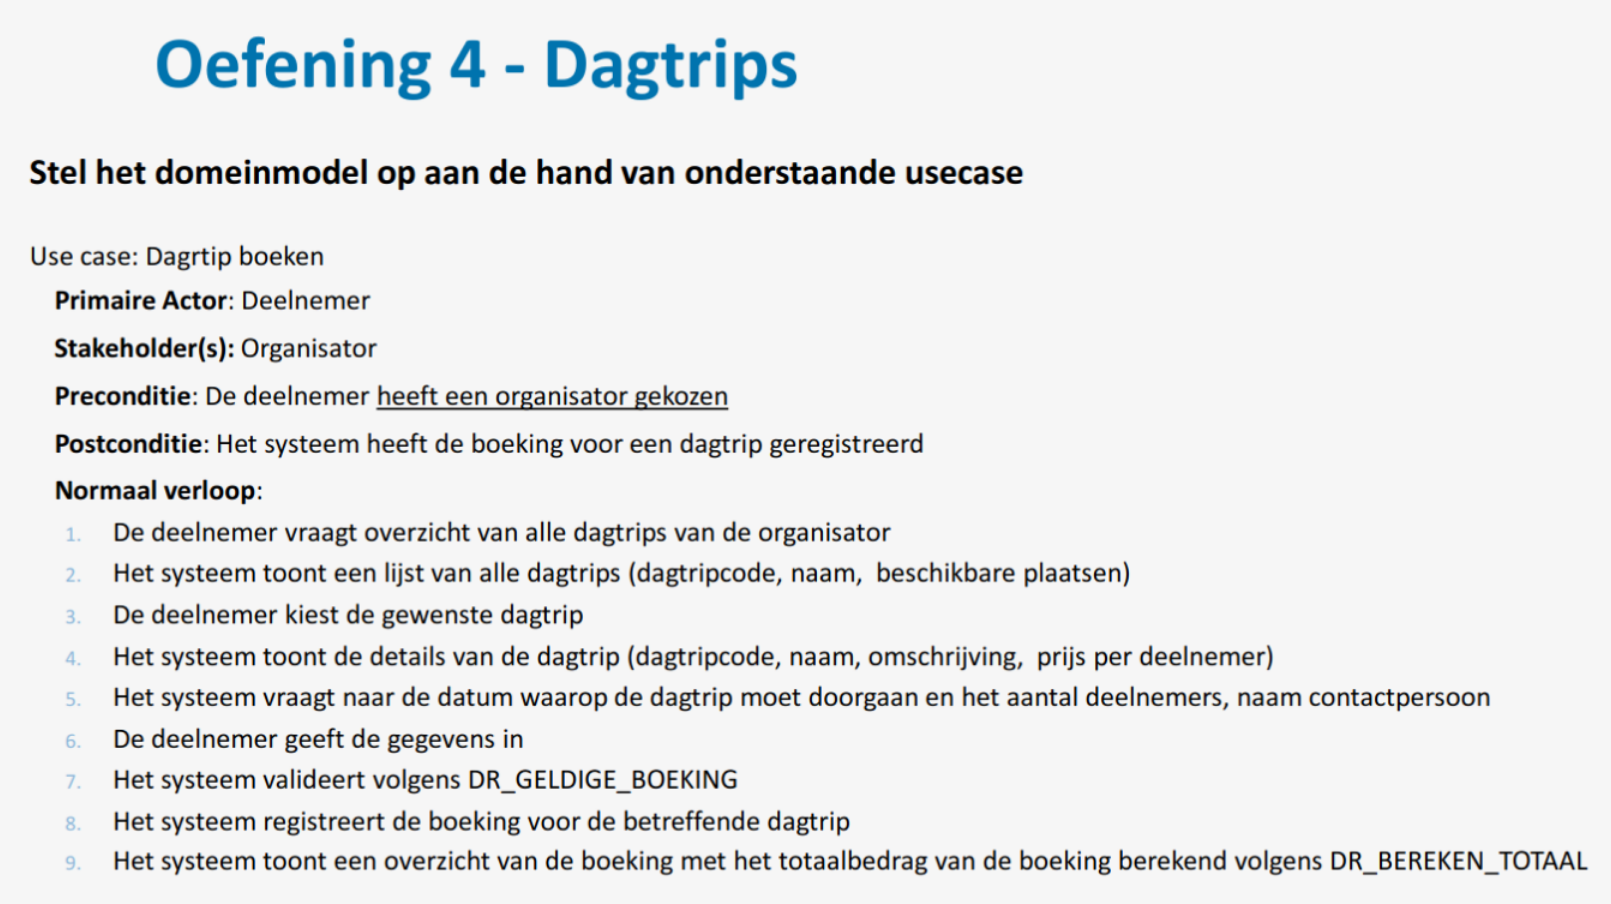
\includegraphics[width=0.6\linewidth]{oef4.png}
\end{figure}

\end{document}

